\documentclass{standalone} % What kind of document this is
\usepackage{tikz} % Import the tikz package
\usetikzlibrary{arrows.meta, positioning}
\tikzset{node distance=2.5cm,
  procstep/.style={ % Sets the properties for each step
    rectangle,
    rounded corners,
    fill=gray!10},
  double distance=2pt, % Adjust appearance of accept states
  every edge/.style={ % Sets the properties for each transition
    draw,
    ->,>=stealth % Makes edges directed with bold arrowheads
  }}
\begin{document}
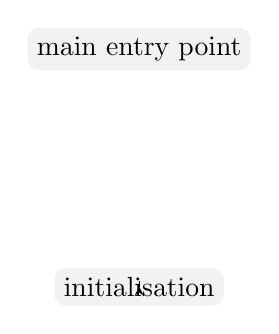
\begin{tikzpicture}
  \node[procstep] (s1) {main entry point};
  \node[procstep, below=of s1] (s2) {initialisation}
    edge [<-] (s2);

    
\end{tikzpicture}
\end{document}